\section{Federated Learning}\label{section:federated_learning}

This section contains necessary background information and context regarding FL.
The first subsection covers fundamental FL building blocks and terminologies.
The next subsection explains vital supplementary FL concepts.
Oakestra orchestrates FLOps.
It uses an unconventional three-tiered structure that allows support for geographical clusters \cite{paper:oakestra_usenix}.
This structure opens up unique opportunities for FL applications.
More advanced FL architectures are necessary to benefit from these opportunities.
The following subsection discusses these architectures.
These three subsections build a solid FL understanding.
A great summary and source of information for deeper insights into the field of FL can be found in \cite{book:fl}.


\subsection{FL Basics}

\begin{figure}[h]
    \centering
    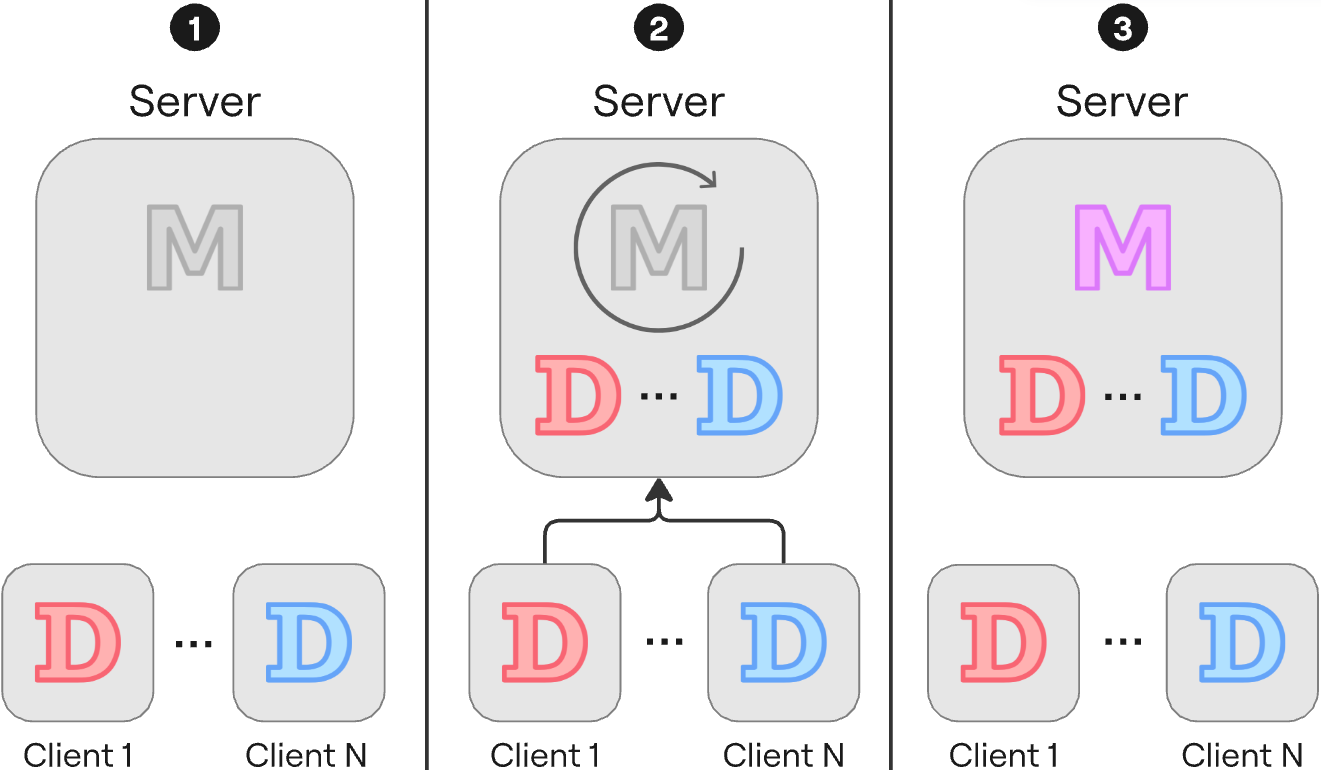
\includegraphics[width=0.9\textwidth]{classic_ml_training.png}
    \caption{Centralized ML Model Training}
    \label{fig:classic_ml_training}
\end{figure}
Figure \ref{fig:classic_ml_training} depicts the classic centralized ML model training process.
Starting from (1), where clients have their data (D) and the server hosts the untrained (gray) ML model (M).
In (2), the clients send their data to the server.
The server can now train the model using data from the clients.
(3) depicts the final state after training.
(The pink/purple model color symbolizes that different data sources have been used during training.)
The client data remains on the server and is exposed to potential exploitation.
As discussed in the introductory chapter, this centralized approach often leads to privacy breaches.

FL was introduced to use sensitive data on client devices for training ML models while keeping that data private.
Thus, FL complies with laws and regulations.
Many different algorithms and strategies exist for FL.
The following example focuses on the widely used base-case/classic FL algorithm FederatedAveraging (FedAvg) \cite{paper:original_fl}.

\begin{figure}%[h]
    \centering
    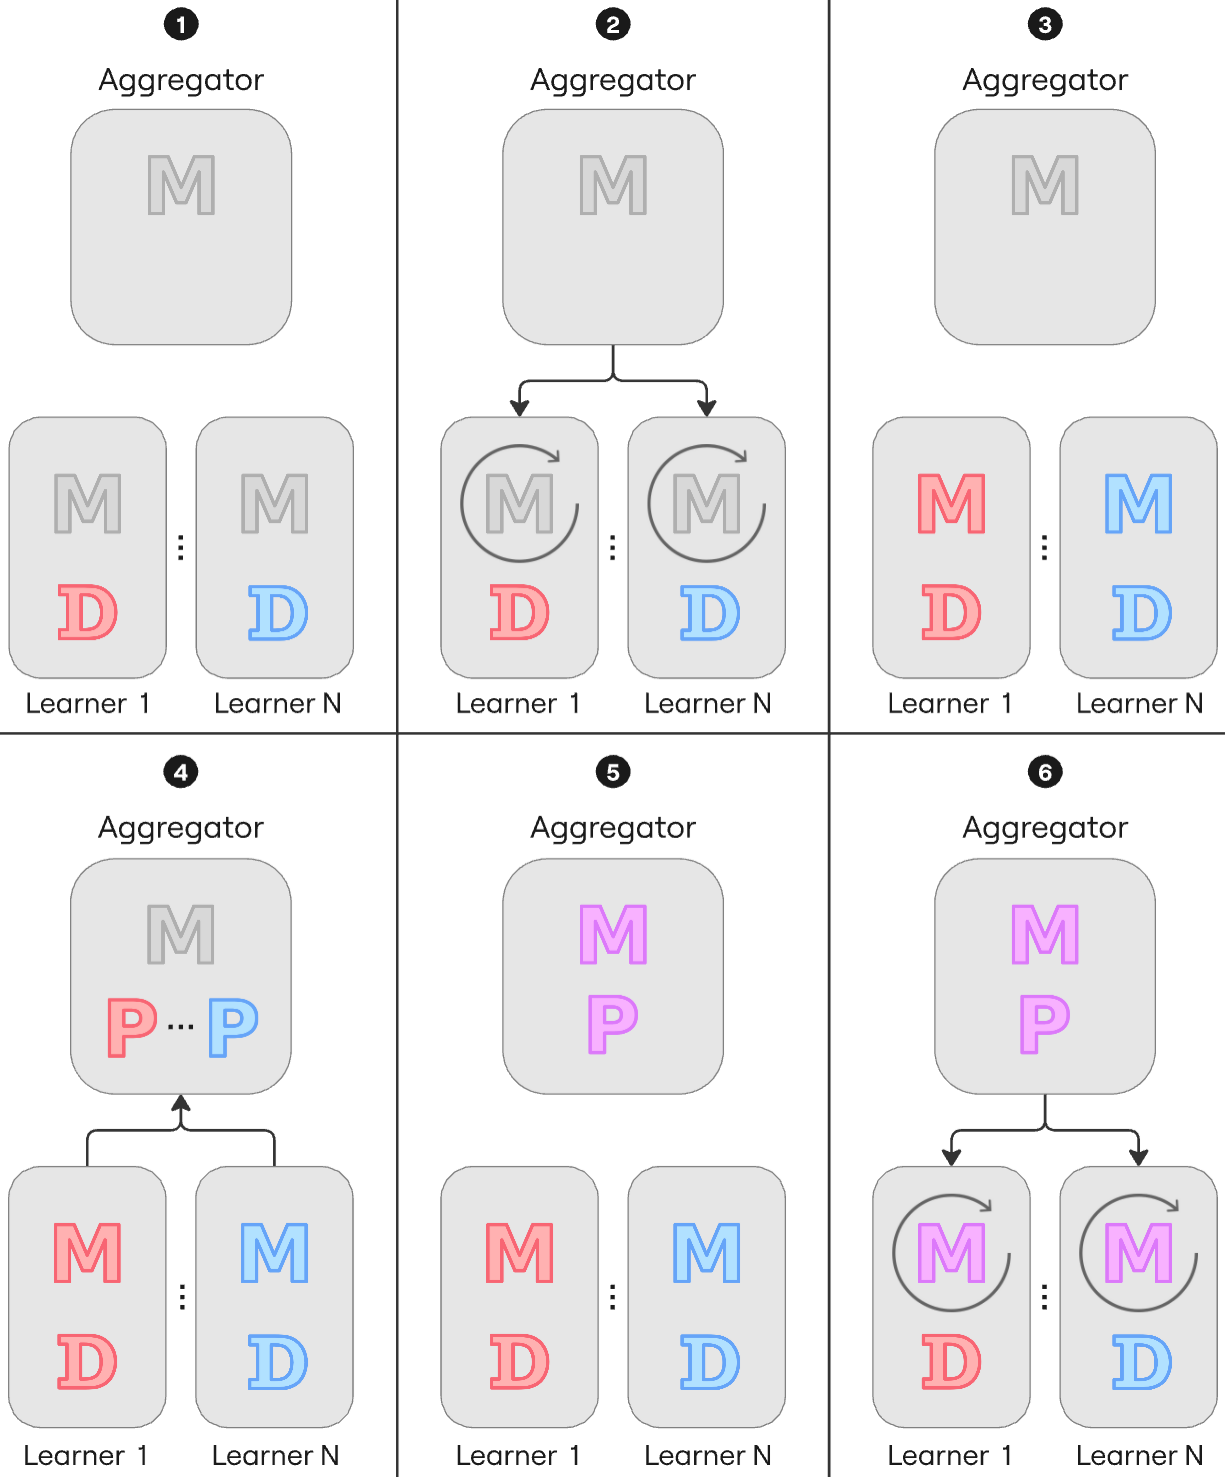
\includegraphics[width=\textwidth]{basic_fl_intro.png}
    \caption{Basic Federated Learning}
    \label{fig:basic_fl_intro}
\end{figure}
Figure \ref{fig:basic_fl_intro} shows the basic FL training loop.
The number of learners can vary.
The first differences are the component names.
In FL, the server is frequently called an \textbf{aggregator}, and it coordinates the FL processes.
Clients are called \textbf{learners}.
Using the terms server and clients in FL is still common
\footnote{
FLOps uses various components, including non-FL servers and clients.
Therefore, this work prefers aggregators and learners because they highlight FL components and help with comprehension.
}.
Another difference is that all components must know and possess the ML model locally.
They also need to set up their environment for training properly.

As a reminder, one can split up ML models into two parts.
One part is (usually) a static lightweight model architecture.
It includes layer specification (in DNNs), training configuration, and hyperparameters like learning step sizes, loss, and activation functions.
Model weights and biases are the dynamic components of an ML model.
A model without them is not useful because weights and biases are what get trained.
They allow the model to fulfill its intended use, such as prediction, inference, or generation tasks.
These weights and biases are the major contributors to a trained model's overall size (space utilization).
Model architecture is static in classic ML/FL.
Thus, FL components can transmit and share weights and biases instead of the entire trained model.
This work calls model relevant data sent between the learners and aggregators (model) \textbf{parameters} and depicts it with (P).

The concrete classic FL steps are as follows.
Initially, at (1), all models are untrained.
At (2), the aggregator starts the first FL training cycle by telling the learners to start their local training.
The local training rounds (epochs) are completed at (3).
(The 'M's are now colored.)
In (4), the learners have extracted their model parameters and sent them to the aggregator.
The aggregator now has access to these parameters but not the sensitive data used to train them.
That is how FL can profit from sensitive data while maintaining its privacy.
Possible attack vectors still exist.
They expose sensitive client information by abusing this parameter-based aggregation process.

In (5), the server aggregates these collected parameters into new global parameters.
This aggregation process is also called model fusion \cite{book:fl}.
The aggregator applies these global parameters to its model instance.
Learners can be heterogeneous and possess varying amounts of data.
Therefore, some learner updates might be more impactful than others.
To respect this circumstance, learners typically also send the number of data samples they used for training to the aggregator.
That way, the aggregator can prioritize its received updates proportionally.
Otherwise, in classic FL aggregation, the mean of the parameters is used for the global model.
The result is a \textbf{global model} that was trained for one FL cycle.

In (6), the aggregator sends its global parameters back to the learners.
The learners apply these parameters to their local model instance to make it identical to the aggregator's global model.
By doing this, learners discard their locally trained parameters.
The FL training loop could terminate, and the learners or servers could use their global model copy for inference.
Otherwise, as depicted in (6), another FL training cycle begins.
There can be arbitrarily many FL cycles, similar to conventional training rounds in classic ML.
FL training eventually terminates due to time/resource constraints or a failure to reach a satisfying performance.
If not terminated, the accuracy and loss will worsen due to overfitting, assuming the available training data is finite and unchanging.

\subsection{Supplementary FL Concepts}

This subsection explores essential supplementary FL concepts to understand the field better.

\subsubsection{FL compared to Distributed Learning}

FL and Distributed Learning (DL) are two related disciplines.
Instead of executing complex ML computations on a centralized resource-rich monolithic machine or data center, both techniques
distribute this computational load among multiple more resource-constrained machines that train individually.
These approaches increase convergence times and avoid needing expensive singular devices with sufficient resources.
After distributively training models, a server aggregates a global model.

The differences between both mechanisms are the following.
FL can use highly heterogeneous non-IID training data.
Quantity and distribution can vary significantly between learners.
FL can handle this varied data without having access to explicit information about their properties before or during training.
FL only utilizes the data that learners offer.
FL can work with a fluctuating number of learners that only participate in a small fraction of training rounds.
This dynamicity leads FL to handle various unique challenges, such as handling errors caused by crashed, failed, or disconnected learners during training.
On the contrary, DL initializes with total centralized access and control to all data before distributing it among its fixed and predefined clients \cite{book:fl}.
DL does not support FL's privacy concerns because it has complete oversight and control of all data.


\subsubsection{FL Variety}
FL is a diverse discipline with various possible applications and use cases.
Most FL work focuses on end-user/edge/IoT devices.
FL is not exclusive to these environments and can work in conventional cloud environments.
As discussed in the first subsection, FL can train DNNs.
FL can also apply to classic ML models, such as linear models (logistic regression, classification, and more) or decision trees for explainable classifications.
FL also supports horizontal, vertical, and split learning.
This work omits discussing these techniques to avoid bloat.
More information about these and other methods is available in \cite{book:fl}.
Plenty of FL optimizations exist for each ML variant, such as custom algorithms and strategies.

Personalization can help if the global model is too general and does not satisfy a learner's individual needs.
Different personalized FL (PFL) approaches exist.
Some take the final trained global model and further train it on local data (fine-tuning).
Other techniques train two local models concurrently.
The first model gets shared and updated with the global parameters.
The second one stays isolated and only gets influenced by local data.
A mixture between the global and purely local model can be used for inference.
PFL is a deep and growing subfield of FL \cite{book:fl,hpfl_over_massive_mobile_edge_computing_networks, paper:adaptive_exper_models_for_pfl}.

\subsubsection{FL Security \& Privacy}
The field of FL prioritizes security and privacy because protecting those was the key motivation for FL's creation.
FL should use secure and authenticated communication channels to prevent messages from being intercepted, read, or impersonated by a man-in-the-middle adversary.
One should ensure that learners and aggregators are the only actors with access to those messages and can decipher them.
A variety of FL adversaries and threats exist.
Fortunately, there exists a growing array of defenses against those threats.
It is crucial to pick and combine these defenses wisely based on the use case and environment.
Two prominent techniques to protect against threats are differential privacy and secure aggregation. \cite{book:fl}

We omit further detailed discussions because FLOps does not focus on privacy or security.

\subsection{FL Architectures}

FL comes in two broad structural categories.
Cross-silo or enterprise FL gets used in large data centers or multinational companies.
Each learner represents a single institution or participating group.
There are only around ten to a few dozen learners involved.
Cross-silo FL considers the identity of the parties for training and verification.
Generally, every individual local update from every learner at every training round is significant.
Fallouts and failures of individual learners are serious.
Cross-device FL can include hundreds or millions of devices, primarily edge/IoT devices.
Due to this great pool of learners, only a subset typically trains per round.
The identities of the participating learners are usually unimportant.
Due to the nature of these devices and their environments, cross-device FL needs to manage special challenges.
Challenges include non-IID data, heterogeneous device hardware, different network conditions, learner outages, or stragglers.
Various techniques exist to navigate these challenging conditions, including specialized algorithms for aggregation or learner selection.
These strategies can consider bias, availability, resources, and battery life.
\vspace{2mm}
\newline\textbf{From now on, when we mention FL in this work, we mean cross-device FL because FLOps focuses on cross-device workloads.}
\vspace{5mm}
\newline
Different FL architectures exist to support large-scale FL environments.
FLOps wants to benefit from the unique three-tiered Oakestra \cite{paper:oakestra_usenix} architecture.
Such a scenario has two main challenges.
The first challenge is managing a massive number of connections and aggregations.
The second one is reducing the negative impact of straggling learner updates.
The problem with using a single aggregator, as seen in \ref{fig:basic_fl_intro}, is that this single aggregator becomes a communication bottleneck.
Additionally, per-round training latency is limited by the slowest participating learner.
Thus, stragglers turn into another bottleneck.
The following is an overview of prominent FL architectures.

\subsubsection{Clustered FL}

\begin{figure}[b]
    \centering
    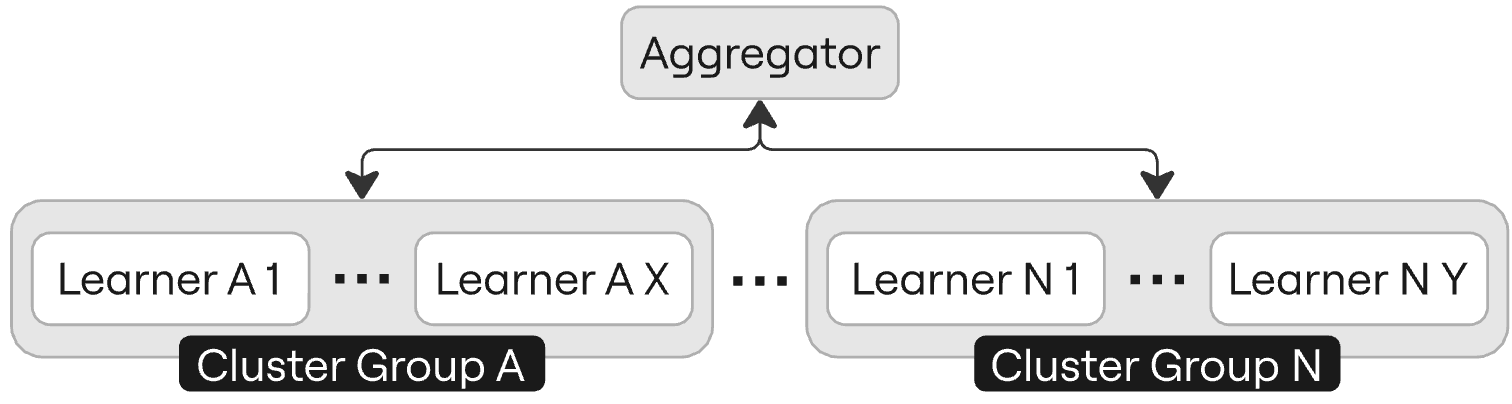
\includegraphics[width=\textwidth]{clustered_fl.png}
    \caption{Clustered FL Architecture}
    \label{fig:clustered_fl}
\end{figure}
Figure \ref{fig:clustered_fl} shows the Clustered FL (CFL) architecture that groups similar learners into clusters.
CFL can form clusters based on local data distribution, training latency, available hardware, or geographical location.
The issue of the singular aggregator as a bottleneck persists.
The main challenge for CFL is choosing a suitable clustering strategy and criteria for the concrete use case.
If the criteria are biased, updates from preferred clusters might be heavily favored, resulting in a biased global model with bad generalization.
Another task is to properly profile the nodes to match them to the correct cluster.
The entire cluster suffers if a slow outlier is present in a cluster.
Node properties can vary over time, so cluster membership has to be dynamic.
Too intrusive profiling can lead to compromised privacy.
The benefits of CFL are its ease of implementation, familiar architecture to classic FL, and flexibility to tune clustering/selection dynamically.
CFL can be combined with other architectures.
A downside of CFL is that a proper clustering strategy is use-case-dependent and challenging to optimize.
CFL does not really solve scalability issues on its own.
Its clustering overhead becomes critical with larger numbers of nodes.
\cite{
    paper:cluster_based_secure_aggregation_for_fl,
    paper:fedat_high_performance_communication_efficient_fl_with_asynch_tiers,
    book:fl,paper:decentralized_edge_intelligence_dynamic_resource_allocation_framework_hfl}

\subsubsection{Hierarchical FL}
\begin{figure}[b]
    \centering
    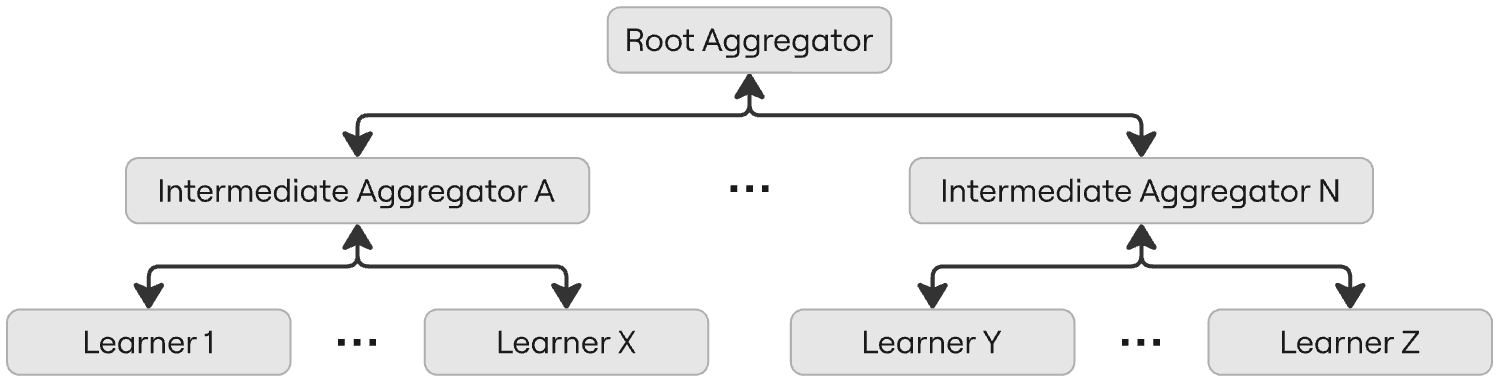
\includegraphics[width=\textwidth]{hfl_architecture.png}
    \caption{Hierarchical FL Architecture}
    \label{fig:hfl_architecture}
\end{figure}
Figure \ref{fig:hfl_architecture} depicts the hierarchical FL (HFL) architecture.
In HFL, the root aggregator delegates and distributes the aggregation task to intermediate aggregators.
HFL can have multiple layers of intermediate aggregators.
Each intermediate aggregator and its connected learners resemble an instance of classic FL.
After aggregating an intermediate model, the intermediate aggregators send their parameters upstream to the root aggregator.
The root combines the intermediate parameters into global ones and sends them downstream for further FL rounds.
HFL's structure requires changing the underlying FL architecture.

The proper design and implementation, and the assignment of learners to aggregators determine the success of one's FL setup.
For example, if too many learners are attached to a given aggregator, that aggregator becomes a bottleneck.
The intermediate aggregated model can be biased if too few learners are assigned.
Thus, the infrastructure resources and management costs become unjustified for the small number of learners.
A management overhead arises with more components, including handling fault tolerance, monitoring, synchronizing, and balancing.
Bad synchronization can amplify straggler problems.
Balancing refers to combining and harmonizing intermediate parameters to get a good global model.
These findings show that special FL architectures, such as HFL, require careful consideration and correct implementation.
\cite{book:fl,paper:decentralized_edge_intelligence_dynamic_resource_allocation_framework_hfl,hpfl_over_massive_mobile_edge_computing_networks}

The benefits of HFL are its dynamic scalability and load balancing.
One can easily add or remove intermediate aggregators and their connected learners.
Due to this distribution of load and aggregation, each aggregator, including the root, is less likely to face bottleneck issues.
One can combine HFL with CFL, where each intermediate aggregator is responsible for one or multiple clusters.
The downsides of HFL are communication and management overheads.
More components lead to more transmitted messages.
These messages all need to be secured and encrypted.
With more components and nodes, adversaries can take advantage of more possible backdoors.
HFL provides a powerful way to improve scalability for FL if done right.
\cite{
    paper:deploying_fl_in_hierarchical_edge_architecture,
    paper:hfl_with_momentum_acceleration_in_multi_tier_networks,
    paper:hfl_with_privacy,
    paper:decentralized_edge_intelligence_dynamic_resource_allocation_framework_hfl,
    book:fl,
    hpfl_over_massive_mobile_edge_computing_networks}


\subsubsection{Decentralized FL}
Decentralized FL does not require a central aggregator.
Instead, it operates on a peer-to-peer basis via a blockchain.
That way, the centralized communication bottleneck gets resolved.
The blockchain represents the global model.
Learners train in parallel.
Each locally trained update gets a version.
Based on this version, random clients are chosen for aggregation.
The results get appended to the blockchain, and the model version is incremented. \cite{book:fl}

\subsubsection{Asynchronous FL}
Asynchronous FL allows learners to train continuously and freely push their updates to the aggregator.
This method eliminates stragglers and dropout problems because a training round does not need to wait or handle outliers and timeouts.
A new issue of staleness arises when updates are merged into the global model that took a very long time to complete.
Such an update used a now outdated version of the global model.
As a result, the global model is partially reverted to an older state.
Asynchronous FL can be combined with other architectures. \cite{book:fl}

\subsection{FL Research}\label{subsection:fl_research}

\begin{figure}[h]
    \centering
    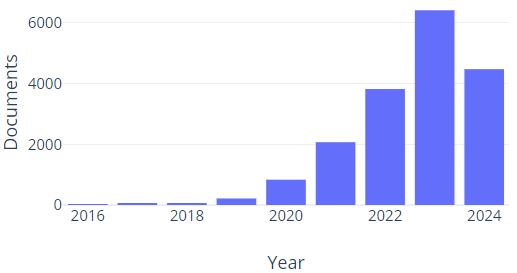
\includegraphics[width=0.8\textwidth]{fl_documents_research.png}
    \caption{Evolution of FL Publications}
    \label{fig:fl_documents_research}
\end{figure}

Figure \ref{fig:fl_documents_research} shows the exponential growth of FL documents since 2016.
(This data comes from searching for "federated learning" in article title, abstract, or keywords via Scopus \cite{scopus_homepage}.)
The idea for this graph is based on \cite{thesis:tum_fl_framework_comparison}.
Graph \ref{fig:fl_documents_research} uses a different query with the latest available data.

Before creating FLOps, we looked for research gaps in the fields of ML at the edge, specifically FL.
We have read and examined 47 papers in detail, with 26 papers focusing on FL. 
Additionally, we consulted several articles, joined and participated in discussion forums, and completed a couple of paid courses.
Discussing each paper in detail would heavily bloat this thesis.
This subsection presents key and meta-findings instead.
While working through the material, we created and incrementally updated a database in which we noted specific properties of each paper.
These properties include one or multiple categories in which the paper fits in.
Additional properties include the initial problems or challenges the authors tried to resolve, their contributions, results, limitations, and envisioned future work.
We also noted what ML or FL frameworks or libraries they claimed to use.

Table \ref{table:fl_research_table_1} depicts a subset of the analyzed FL papers.
It presents the documented contributions, limitations, and future work properties.
The remaining FL papers are available in Appendix \ref{appendix:fl_research}.
Note that we omit some of the 26 FL papers from these tables because we discuss them in greater detail throughout the background section.
These tables provide a good impression of the examined FL papers.
The following is a broad aggregated overview of a subset of these papers and their technical outcomes.
More precise individual insights of the examined paper are available in the mentioned tables.
Several papers \cite{paper:fl_inference_anytime_anywhere,paper:hfl_with_momentum_acceleration_in_multi_tier_networks,paper:model_pruning_for_edge_fl,paper:tackling_objective_inconsistency_problem_in_heterogeneous_fl} proposed novel learning methods that improve handling non-IID data, reduce resource usage, improve model quality, or train models quicker than previous methods.
Besides inventing or improving learning methods, others \cite{paper:refl_resource_efficient_fl,paper:edge_fl_via_mqtt_and_oma_lightweight_m2m,paper:fedat_high_performance_communication_efficient_fl_with_asynch_tiers} focus on new learner selection or aggregation algorithms to benefit the most from the available resources, especially from heterogeneous data.
Many works \cite{paper:edgefl_framework,paper:global_fl_platform_for_iot,paper:adaptive_exper_models_for_pfl} investigate the benefits and downsides of using different architectures for FL that lead to more efficient, performant, and scalable FL.
Other works \cite{paper:hfl_with_privacy, paper:cluster_based_secure_aggregation_for_fl,paper:efficient_privacy_preserving_ml_in_hierarchical_distributed_systems} focus on new privacy and security schemas or improve existing secure aggregation algorithms to reduce existing overheads and bottlenecks when using conventional protection.
A large portion of the examined works investigated and proved novel concepts to achieve a range of goals, from better privacy, scalability, and less overhead to better resource utilization.
Examples include \cite{paper:decentralized_edge_intelligence_dynamic_resource_allocation_framework_hfl,hpfl_over_massive_mobile_edge_computing_networks,paper:fl_toward_on_demand_client_deployment_at_edge}.
Patterns and trends can be extracted from these papers based on the documented properties.

\begin{figure}[p]
    \begin{changemargin}{-2cm}{0cm}
    \begin{tabular}{|c||m{0.4\paperwidth}|m{0.4\paperwidth}|}
        \hline
            ID & Contributions & Limitations \& Future Work \\
        \hline
            \cite{paper:refl_resource_efficient_fl}
            &
            A novel selection and staleness-aware aggregation strategy.
            Analysis of resource wastage and the impact of stragglers.
            A smart participation selection based on learner availability.
            &
            Privacy or security were not considered.
            Evaluations are based on classic datasets (MNIST, CIFAR-10), which do not reflect real non-IID data.
            Only homogeneous resources were assumed.
            Use of a simple linear regression model for availability prediction.
            More sophisticated alternatives exist.
            Factors such as battery level, bandwidth, and user preferences should also be considered for availability prediction.
        \\
        \hline
            \cite{paper:cluster_based_secure_aggregation_for_fl}
            &
            A novel cluster-based secure aggregation strategy for diverse nodes.
            Clustering based on processing score \& GPS information/latency leads to better throughput and reduces false-positive dropouts.
            A new additive sharing-based masking scheme that is robust against dropouts.
            &
            All participants are assumed to be honest.
            Malicious users were not considered.
            The aggregator might become a bottleneck, which can be resolved via HFL (with cluster heads).
            Image classification was the only evaluated ML task.
        \\
        \hline
            \cite{paper:privacy_preserving_deep_fl_for_coop_hierarchical_caching_in_fog_computing}
            &
            An FL caching scheme including novel algorithms and architecture.
            Utilization of an AI training model that considers user history.
            &
            A convergence analysis was not provided.
            For further security and privacy improvements, blockchain-empowered FL should be investigated.
        \\
        \hline
            \cite{paper:model_pretraining_and_initialization_for_fl}
            &
            Analysis of the impact of pre-training ML models for FL initialization compared to the common random approach.
            Findings show pre-trained model superiority.
            &
            It is challenging to get a pre-trained model if the necessary data is not available or private.
            Using pre-trained models can lead to biases.
            Only a specific (warm-start) initialization strategy was considered.
        \\
        \hline
            \cite{paper:decentralized_edge_intelligence_dynamic_resource_allocation_framework_hfl}
            &
            A novel incentive/resource-based allocation schema that utilizes game theory.
            Learners with more data are more valuable and they can compete for higher participation rewards.
            Multiple model owners compete for cluster heads with the most data.
            &
            The effects of social networks and their impact on worker's cluster selection decisions should be researched.
            Malicious workers were not considered.
        \\
        \hline
            \cite{paper:fedat_high_performance_communication_efficient_fl_with_asynch_tiers}
            &
            Synergy of asynchronous and synchronous FL via asynchronous tiers, which is able to handle stragglers.
            &
            The tiers all update the server individually.
            Further improvements are possible via HFL with intermediate cluster heads to do the aggregation.
            Additional security could be applied at these cluster heads.
        \\
        \hline
    \end{tabular}
    \captionof{table}{FL Papers considered for FLOps - Part I} 
    \label{table:fl_research_table_1}
\end{changemargin}

\end{figure}

\begin{figure}[p]
    \centering
    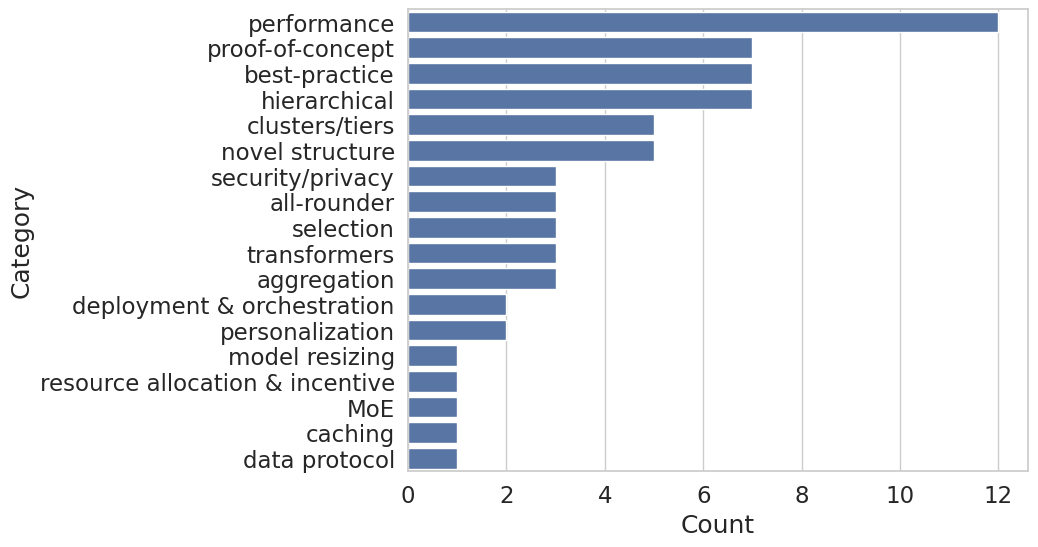
\includegraphics[width=1.0\textwidth]{fl_research_categories.png}
    \caption{FL Paper Categories}
    \label{fig:fl_research_categories}

    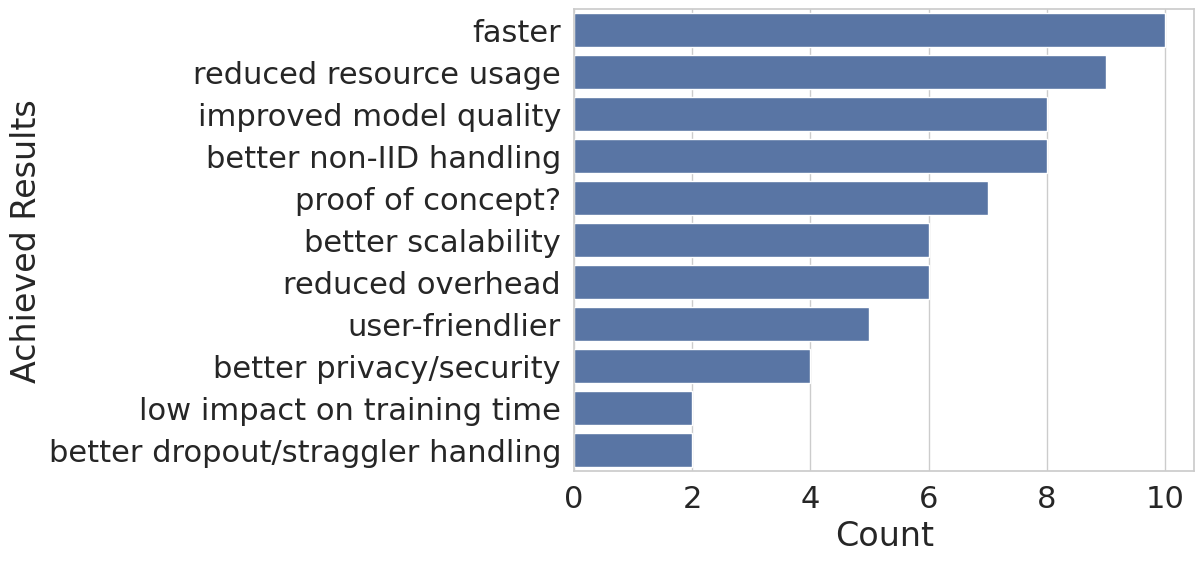
\includegraphics[width=0.9\textwidth]{fl_research_achieved_results.png}
    \caption{Achieved Results of FL Papers}
    \label{fig:fl_research_achieved_results}
\end{figure}

Patterns and trends help to better understand the research field of FL as a whole.
Figure \ref{fig:fl_research_categories} shows the different categories and their distribution.
Most examined papers focused on performance, trying new concepts, finding best practices, and exploring different FL architectures.
Only two papers focused on deployment and orchestration.

The achieved results match these categories.
Figure \ref{fig:fl_research_achieved_results} shows that these contributions lead to more efficient FL.
Improved aspects include speed, resource utilization, training results, and handling of heterogeneous data.
Additional insights about the research problems, contributions, limitations, and future work of the examined FL papers are available in the appendix \ref{appendix:fl_research}.

These documented properties might be biased, and the inspected sample size of papers is relatively small.
To improve confidence in these findings, we compare them with the total number of published works about FL.
Figure \ref{fig:fl_publications_compared} depicts how many works have been published in FL with specific keywords that match our custom categories.
We applied the same method to gather the data as for \ref{fig:fl_documents_research}.
The global results paint a similar picture as our samples.
The most popular topics in FL are related to privacy/security, performance, or algorithms.
Only a tiny portion of FL papers focus on usability, automation, orchestration, or other initial steps.

It seems that researchers assume others to already have working FL environments.
Furthermore, they seem to motivate their readers to optimize these setups based on their findings instead of replicating and configuring such an FL setup initially.
These tendencies are visible when inspecting the ML and FL frameworks and libraries the authors mentioned they used.
The following figure is again based on our examined papers.
Figure \ref{fig:fl_research_ml_and_fl_frameworks} shows that most authors did not explicitly state what ML framework or library they used for their work.
Many researchers used Pytorch and TensorFlow.
The figure also shows that FL researchers rarely mention what FL frameworks they use for their work.
It is much more common for authors to mention what ML framework they used than what FL framework they used.
Possible reasons for this might be that ML as a field is a lot older, more sophisticated, widespread, and established.
The same applies to ML frameworks.
On the other hand, FL is a very young subfield of ML research.
FL frameworks are still in their early stages.
FL researchers might be using FL frameworks.
However, due to the framework's immaturity, the researchers might not deem it important to explicitly point out that they used them.
Another possible explanation is that FL researchers are experts in FL and can set up and configure FL from the ground up.
Either way, this lack of transparency makes reproducing or extending their work challenging, if not infeasible.
These gaps in FL research motivated the creation of FLOps.

\begin{figure}[p]
    \centering
    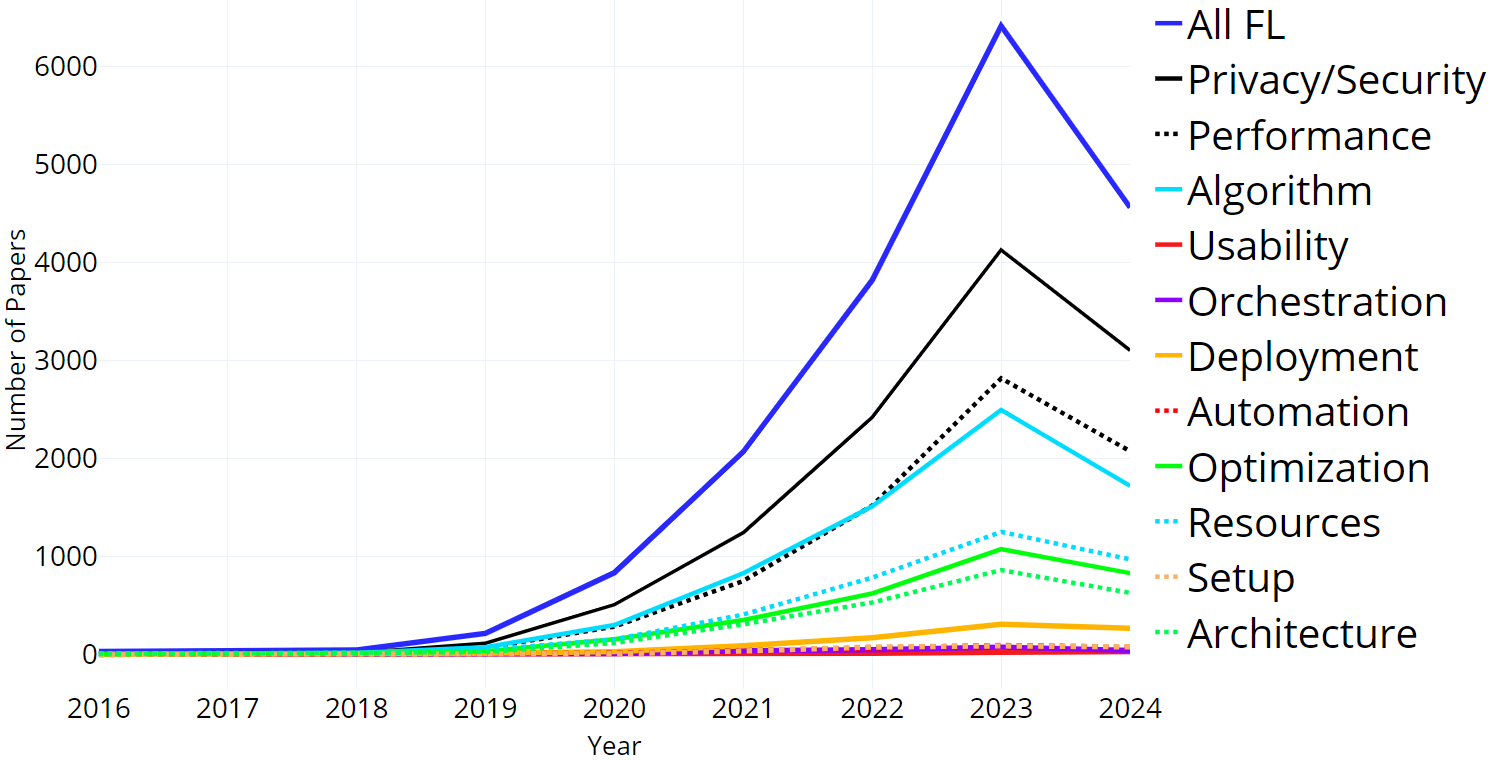
\includegraphics[width=1.0\textwidth]{fl_publications_compared.png}
    \caption{Evolution of FL Publications based on Keywords}
    \label{fig:fl_publications_compared}
    \vspace{2cm}
    \begin{adjustwidth}{-0.1\paperwidth}{-0.1\paperwidth}
        \centering
        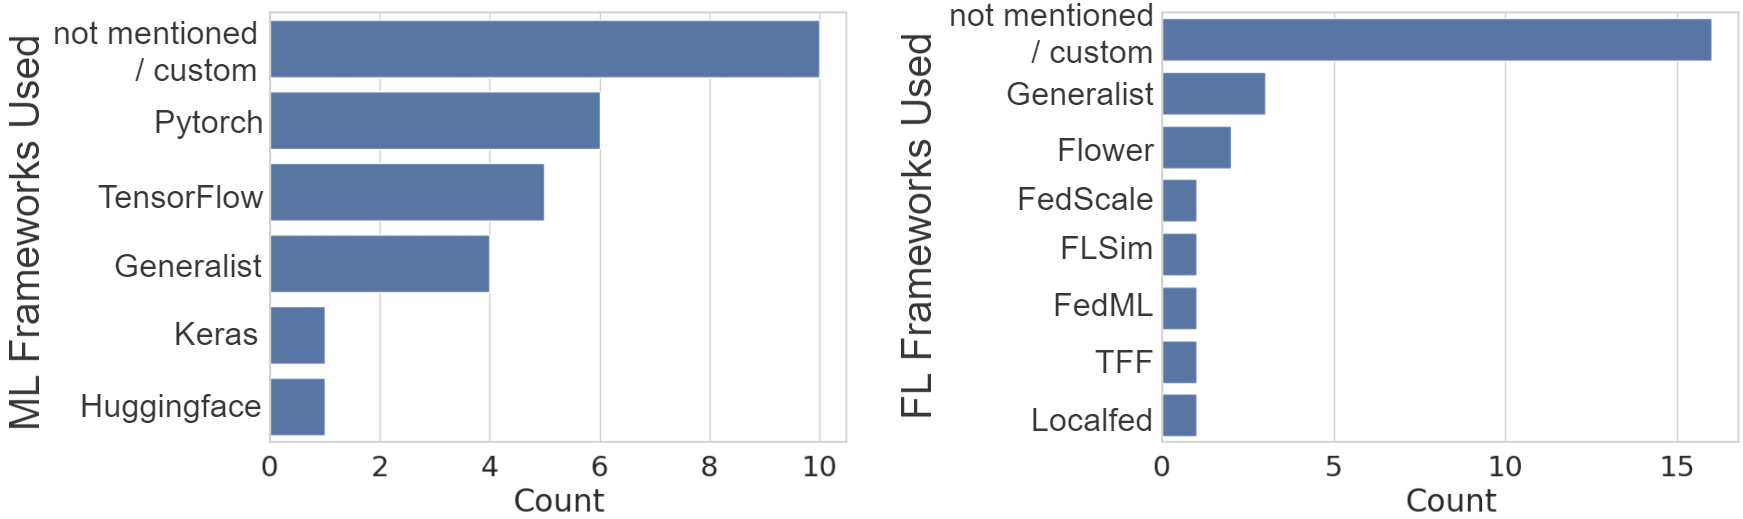
\includegraphics[width=0.8\paperwidth]{fl_research_ml_and_fl_frameworks.png}
        \caption{Distribution of mentioned ML and FL Frameworks in FL Papers}
        \label{fig:fl_research_ml_and_fl_frameworks}
    \end{adjustwidth}
\end{figure}

\pagebreak
\subsection{FL Frameworks \& Libraries}\label{subsection:fl_frameworks_and_libraries}

\begin{figure}[b]
    \begin{changemargin}{0cm}{0cm}
    \centering
    \begin{tabular}{|m{2.4cm}||c|c|c|c|c|c|}
        \hline
            \textbf{Framework} & \textbf{Version} & \textbf{Releases in 2024} & \textbf{Stars} & \textbf{Forks} & \textbf{Open Issues} \\
        \hline
            Pysyft \cite{fl_framework:pysyft} & 0.9.0 & 62 & 9.4k & 2k & 2
        \\
        \hline
            Tensorflow Federated \cite{fl_framework:tensorflow_federated} & 0.85.0 & 18 & 2.3k & 578 & 168
        \\
        \hline
            FedML \cite{fl_framework:fedml} & 0.8.9 & 0 & 4.1k & 776 & 118
        \\
        \hline
            Flower \cite{fl_framework:flower} & 1.10.0 & 4 & 4.7k & 815 & 284
        \\
        \hline
            OpenFL \cite{fl_framework:openfl} & 9.3.4 & 2 & 1.9k & 426 & 256
        \\
        \hline
    \end{tabular}
    \captionof{table}{Updated FL Framework Comparison} 
    \label{table:updated_fl_framework_comparison}
\end{changemargin}

\end{figure}

This subsection examines the current landscape of available FL frameworks.
The goal is to better comprehend why most researchers did not specify or use FL frameworks in the previous findings.
This discussion will be brief because Saidani already analyzed and evaluated FL frameworks in great detail in his master's thesis \cite{thesis:tum_fl_framework_comparison} from 2023.
He examined FL libraries, frameworks, and benchmarks.
Many FL tools exist for specific niche use cases and architectures \cite{thesis:tum_fl_framework_comparison}.
This finding contradicts the opinions of his questioned FL practitioners and experts.
They expected FL libraries and frameworks to focus on basic FL features, such as communication, aggregator-learner orchestration, security, and data aggregation.
Many libraries and frameworks, most of which were not production-ready, were still in an experimental research state \cite{thesis:tum_fl_framework_comparison}.

To reduce complexity, he focused on the five most promising open-source frameworks.
For a framework to be allegeable, it had to fulfill 2/3 of the following criteria.
It needed more than one thousand starts and 350 forks on GitHub.
The interviewed experts had to mention it.
The framework had to support all major operation systems.
Because FL is rapidly evolving, we updated his findings and expanded upon them.
We included the number of releases (including patches) in 2024 so far and the number of open issues in the repository.

Table \ref{table:updated_fl_framework_comparison} shows the updated FL Framework comparison (16.08.2024).
These FL frameworks are in active development. 
Only FedML has not been updated for several months now.

Saidani's main original contribution was a novel FL benchmarking suite called FMLB (Federated Machine Learning Benchmark).
Its goal was to evaluate and compare the mentioned FL frameworks efficiently.
His previous analysis and summary of existing frameworks were sound and helpful.
However, we are critical of his evaluation results, especially the poor performance of Flower.
We tried to replicate his experiments, but his provided code \cite{tum_fl_framework_thesis_github} lacks instructions on how to set up this benchmark application.
We simulated the experiments with the latest official flower version at the time and made sure to stick as closely as possible to the same experimental setup and configuration.
Our findings show very different results.
Flower manages to solve the experiment quickly and efficiently.
Our results match the verdicts of other works comparing FL frameworks, such as \cite{comparative_analysis_of_fl_frameworks} or \cite{comprehensive_study_fl_frameworks_degree_project}.
\cite{comparative_analysis_of_fl_frameworks} is the latest work that compares FL frameworks that we considered, and its verdict is that Flower outperforms all its competition.
FLOps uses Flower as its FL framework of choice.
\subsection{Flower} \label{subsection:flower}

Flower \cite{paper:flower} is a research-backed open-source FL framework.
One major target in Flower's paper was to narrow the gap between research and production.
It allows researchers to run high-performance FL simulations and rapidly transition to tangible production environments using the same tool.
Another focal point of its paper was scale and parallelization.

Flower is a sophisticated, feature-rich FL framework.
Flower's first release (0.10.0) was published in November 2020, and its first major release (1.0.0) was published in 2022 \cite{fl_framework:flower}.
Flower supports all major operating systems, containerization, and ML libraries.
It aims to be easily customizable and extendable via a programming language and ML framework agnostic design.
Flower strives to offer all popular FL features, such as support for different data types and distributions.
Further features include pre-implemented popular FL algorithms and vertical and horizontal data splitting support.
Flower supports traditional ML tasks, like regression or clustering, DNNs, LLMs, and security mechanisms, such as secure aggregation.
It enables the use of FL via CPUs or GPUs.
The default communication protocol is gRPC, which can be replaced.
Flower supports various FL variants, including PFL, edge computing, cross-silo, and cross-device.
It handles and implements core FL components but does not handle many other aspects, like deployment, orchestration, dependency management, or containerization.
Flower offers a mature set of FL simulation techniques.

Users can easily change and add functionality to the framework by interacting with flexible abstractions and interfaces.
The heart of Flower is its strategy concept.
The aggregator uses this strategy to manage the FL processes.
A strategy contains all necessary configurations, such as the FL algorithm and the minimum number of learners required for training or evaluation.
Users can pick from more than 30 existing strategies \cite{flower:strategies} or extend from basic strategies and develop their own behavior.
It does not have native out-of-the-box support for model pruning, advanced security/privacy techniques, CFL, HFL, MLOps, or orchestration.
Due to Flowers' flexible design, users can implement their custom features and strategies based on the available basic Flower components.

It is straightforward to set up Flower and start working with it.
Flower is directly available via Python's default package manager pip.
One has to define the server/aggregator, strategy, and clients/learners.
Users can implement the simplest case with a few dozen lines of Python code.
The crucial part is to configure the strategy and clients properly.
One needs to create a client class that extends from a Flower client and implement four essential methods that the framework will call during training.
These methods include a getter and setter for the model parameters and one method each for training/fitting and evaluating the model.
In conclusion, Flower provides a rapid and easy onboarding experience.

Flower has a modern, user-friendly, growing ecosystem.
A dedicated sub-project called Flower Datasets \cite{flower:datasets} is part of this ecosystem.
This project is still in its infancy (v0.3.0).
It allows users to pull HuggingFace \cite{hugging_face_homepage} datasets easily and split them into FL-optimized data fragments.
Users can configure how to split this data up.
Flower Datasets can turn standard non-federated homogeneous/IID datasets into challenging, federated, non-IID data, which is ideal for FL research and development.
This ecosystem includes a well-structured and rich homepage \cite{flower:homepage}, an extensive set of tutorials, guides, example projects \cite{flower:examples}, and documentation \cite{flower:homepage_docs, flower_docs} that ranges from beginner-friendly to advanced.
They have open monthly community events \cite{flower:monthly}, yearly summits \cite{flower:summit}, a blog \cite{flower:blog}, a discussion forum \cite{flower:forum}, a Slack space \cite{flower:slack}, and a YouTube channel \cite{flower:youtube}.